\documentclass[a4paper,10pt]{article}
\usepackage[utf8]{inputenc}
\usepackage{ngerman}
\usepackage{mathtools}
\usepackage{tikz}
\usepackage[backend=biber,style=numeric,bibstyle=authortitle,sorting=none]{biblatex}
\begin{filecontents*}[overwrite]{general.bib}
@conference{rodrigues:scheme_matching_alma,
  author = {Diego Rodrigues and Altigran da Silva and Rosiane Rodriguesm and Eulanda dos Santos},
  year = {2015},
  title = {Using active learning techniques for improving database schema matching methods},
  booktitle = {2015 International Joint Conference on Neural Networks (IJCNN)}
}

@conference{jiuzhen:xml_schema,
  author = {Zhao Jiuzhen and Zhang Shidong and Yan Zhongmin},
  year = {2009},
  title = {A Novel Method for XML Scheme Matching},
  booktitle = {2009 International Forum on Information Technology and Applications}
}

@conference{gou:source_xml,
  author = {Heping Gou and Yongxia Jing and Baiming Feng and Yong Li},
  year = {2012},
  title = {A Scheme of Information Integration Based on XML Description and Schema Matching},
  booktitle = {2012 Fourth International Conference on Computational and Information Sciences}
}

@conference{boettcher:data_mapping,
  author = {Stefan Böttcher and Sven Groppe},
  year = {2003},
  title = {Automated data mapping for cross enterprise data integration},
  booktitle = {2003 International Conference on Enterprise Information Systems}
}

@online{dozer:dozer,
  year = {2019},
  title = {Dozer},
  url = {https://github.com/DozerMapper/dozer},
  urldate = {2020-02-02}
}

@online{halterman:modelmapper,
  author = {Jonathan Halterman},
  year = {2019},
  title = {modelmapper},
  url = {http://modelmapper.org/},
  urldate = {2020-02-02}
}

@online{adverity:adverity,
  year = {2020},
  title = {Adverity},
  url = {https://www.adverity.com/analytics-platform/data-integration/},
  urldate = {2020-02-02}
}

@online{altova:mapforce,
  author = {Altova},
  year = {2020},
  title = {Datenmapping-Tools},
  url = {https://www.altova.com/de/mapforce},
  urldate = {2020-02-02}
}
\end{filecontents*}

\addbibresource{general.bib}

%opening
\title{BinClassifier}
\author{Marcus Schlutter - 5098826\\marcus.schlutter@siemens.com}

\begin{document}

\maketitle

\section{Abstrakt}
Vorgestellt wird ein nicht-deterministisches Verfahren, dass Werte aufgrund ihrer abstrakten Pfade in
unterschiedlichen Repräsentationen verknüpft um daraus ein ``Bauanleitung'' ableiten zu können. Mit
einem Demonstrator wurde aus der gelernten Beziehung zwischen einer xml- und einer xlsx-Datei die
xml-Datei rekonstruiert.

\section{Motivation}
\label{sec:motivation}
In den 90er Jahren begann die breitflächige Digitalisierung der Büroarbeitsplätze und doch findet sich auch
heute noch genug ''Handarbeit'' im Büro. So wird z.B. bei Siemens noch immer die GSDML (ein spezielisiertes
XML-Dokument) manuell mit den in Excel-Dateien vorliegenden Gerätespezifikationen gepflegt. Der
Automatisierung des Prozesses steht der große strukturelle Unterschied in der Organisation der Informationen
in beiden Dateiformaten im Wege. Um diese Hürde nehmen zu können wird hier ein nicht-deterministischer
Ansatz vorgeschlagen.

\section{Allgemeiner Ansatz}
Im Gegensatz zu bestehenden Software-Werkzeugen, die für ähnliche Aufgaben angestellt werden, soll die
Assoziation der zugrunde liegenden Daten mit ihrer Bedeutung aufgegeben werden und durch einen
repräsentierenden\\(Navigations-) Pfad innerhalb der Datei ''abstrahiert'' werden. Alle Pfade, die
die selbe Information in beiden Dateien reproduzieren konnten werden im \textit{BinClassifier}, der eine
Liste von Pfad-Histogrammen bzw. ein 2-dimensionales Histogramm als Speicherstruktur aufspannt gespeichert.
Gesammelt wird die Häufigkeit des Auftretens von Paarungen in vorzugsweise ein-eindeutigen ''Töpfen''
(Bins), wie in Abb. \ref{classifier_table} angedeutet.

\begin{figure}[h]
 \centering
 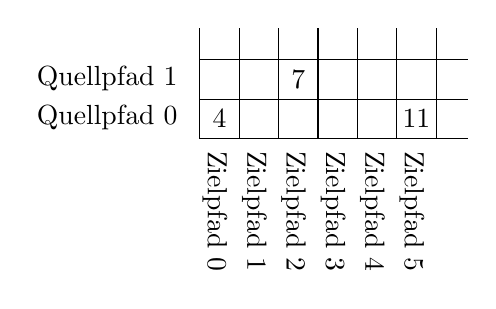
\begin{tikzpicture}
  \draw (1,2.4) -- (1,1) -- (4.4,1);
  \draw[step=0.5] (1,1) grid (4.4,2.4);
  \foreach \x/\i in {1.1/0, 1.6/1, 2.1/2, 2.6/3, 3.1/4, 3.6/5}
    \node[label={[label distance=1, text depth=-1ex,rotate=-90]right: Zielpfad \i}] at (\x,1) {};
  \foreach \y/\i in {1.3/0, 1.8/1}
    \node[label={[label distance=1, text depth=-1ex]left: Quellpfad \i}] at (1,\y) {};
  \node at (1.25,1.25) {4};
  \node at (2.25,1.75) {7};
  \node at (3.75,1.25) {11};
 \end{tikzpicture}
 \caption{2-dimensionales Histogramm als Speicherstruktur}
 \label{classifier_table}
\end{figure}

Dafür müssen einige Anforderungen an die zugrunde liegenden Daten formuliert werden: alle vorzufindenden
Datenklassen\footnote{eine Datenklasse ist eine (gedachte) Datenstruktur, die mehrere Datenpunkte unter
einem Namen vereint und in signifikanter Anzahl in der Quelldatei vorkommt: Beispiele in der GSDML sind
DeviceAccessPointItem und ModuleItem} müssen in ihrer Struktur homogen sein, während die Werte über die
Mitglieder einer Klasse heterogen sein müssen. Für die Anzahl der Klassenattributwerte muss dabei gelten:
\begin{displaymath}
 \lvert V \rvert \ll \lvert A \rvert \cap \lvert B \rvert
\end{displaymath}
wobei $A$ und $B$ die Menge der Werte zweier unterschiedlicher Attribute einer Datenklasse darstellt.\newline
Außerdem sollten sich etwaige Fehler in beiden Dateien nach der geometrischen Häufigkeitsverteilung
verteilen, so für ein Attribute $A_i$ der Attributmenge $A$ gilt:
\begin{displaymath}
 P_{mismatch} (A_i) = P_{\lvert A\rvert \cap\lvert B\rvert} + P_{geom} \ll 50\%
\end{displaymath}

\section{Trainingsprozess}
Für das Training werden Paare aus aus Werten und Identifizierern der unterschiedlichen Instanzen der
Datenklasse(n) unter einem Navigationpfad aus der Quelldatei entnommen. Der Quellpfad wird im
Classifier registriert und es wird jeder erfolgreiche Versuch ein Wert-Name-Paar unter einem
Navigationspfad aus der Zieldatei registriert bzw. inkrementiert. Um den Signal-Rausch-Abstand zu
erhöhen können für den Zielpfad zusätzliche Voraussetzungen definiert werden.

\section{Vorteile}
Durch die Abstraktion zu Pfaden wird die Begrenzung durch unterschiedliche Datenstrukturen aufgebrochen,
was es dem Algorithmus erlaubt, sich auf Änderungen einzustellen und durch erneutes Training auf
Strukturänderungen einzugehen: so soll das bishergen ''händische'' pflegen von der GSDML weitestgehend
eleminiert werden. Gleichzeitig kann das abgeleitete 2-dimensionale Histogramm von einem Menschen
interpretiert werden und notfalls von einem Menschen korrigierend eingegriffen werden. Neuronale Netze,
die sonst bei ähnlichen Aufgabenstellungen eingesetzt werden bieten diesen Einblick nicht.

\section{Verwandte Technologien}
Die vorgestellte Lösung sollte wohl zwischen den Forschungsfeldern \textit{scheme matching} und
\textit{value matching} einzuordnen sein: während sich anhand von \cite{rodrigues:scheme_matching_alma}
oder \cite{gou:source_xml} erkennen lässt, dass sich scheme matching auf das Finden von Feldern
mit gleichem Inhalt anhand eines Ähnlichkeitsfaktors in Datenbanken (und ähnlich eindimensionalen
Datenstrukturen) konzentriert, behandelt das value matching das Finden von selben Werten in komplexen
Datenstrukturen. Kommerzielle Lösungen beschränken sich dabei auf ``matching'' in Datenstrukturen
einer Programmiersprache (z.B. \cite{dozer:dozer} oder \cite{halterman:modelmapper}) oder um ein manuelles
mapping mittels grafischer Werkzeuge, wie z.B. in \cite{adverity:adverity} oder \cite{altova:mapforce}.\newline
Einzig in \cite{boettcher:data_mapping} scheint sich eine ähnliche Zielstellung zu befinden: allerdings war
zum Zeitpunkt der Erstellung kein Zugriff auf das Dokument möglich.

\section{Implementierung}
Im Rahmen der Konzeptionierung wurde ein Proof-of-concept in Python realisiert, der mit einer in seiner Struktur
extrem vereinfachten Version einer GSDML bzw. Spezifikation in Excel konfrontiert wurde. Durch zusätzliche
Beschränkungen, wie z.B. einen farblich abgetrennten Tabellenkopf konnte bei fehlerfreien Ausgangsdateien eine
fast eindeutige Pfadzuordnung erreicht werden, wie Abb. \ref{classifier_ex} entnommen werden kann.
\begin{figure}[h]
 \centering
 \includegraphics[scale=0.4]{example_table}
 \caption{Pfadzuordnung der Daten aus dem Proof-of-concept mit 20 Arbeitern. An der Seite stehen die Pfade aus
          der XML-Datei, im Tabellenkopf stehen die Pfade aus den Excel-Dateien}
 \label{classifier_ex}
\end{figure}
Für die Implementierung des Projektes hat sich eine Trennung der Aufgaben nach Dateien und dem Classifier angeboten.
Um zwischen den 3 Modulen zu vermitteln wurde noch ein zusätlicher Managing-Layer eingezogen: die Projektorganisation des Proof-of-concept kann Abb. \ref{project_structure} entnommen werden.
\begin{figure}
 \centering
 \includegraphics[scale=0.5]{ProjektStruktur}
 \caption{Prinzipieler Aufbau des Proof-of-concept in Modulen}
 \label{project_structure}
\end{figure}

\section{Zusammenfassung}
Vorgestellt wurde der so getaufte \textit{Bin-Classifier}, dessen Neuerungen darin bestehen, dass Werte unabhängig
von ihrer Bedeutung auf Navigationpfade abstrahiert werden und in einem 2-dimensionalen Histogramm gesammelt werden.
Um Änderungen aus der Zieldatei in die (oder eine neue) Quelldatei zu übertragen müssen nur noch die Pfade-Paare
interpretiert werden.


\printbibliography

\end{document}
